% mnras_template.tex 
%
% LaTeX template for creating an MNRAS paper
%
% v3.0 released 14 May 2015
% (version numbers match those of mnras.cls)
%
% Copyright (C) Royal Astronomical Society 2015
% Authors:
% Keith T. Smith (Royal Astronomical Society)

% Change log
%
% v3.0 May 2015
%    Renamed to match the new package name
%    Version number matches mnras.cls
%    A few minor tweaks to wording
% v1.0 September 2013
%    Beta testing only - never publicly released
%    First version: a simple (ish) template for creating an MNRAS paper

%%%%%%%%%%%%%%%%%%%%%%%%%%%%%%%%%%%%%%%%%%%%%%%%%%
% Basic setup. Most papers should leave these options alone.
\documentclass[fleqn,usenatbib]{mnras}

% MNRAS is set in Times font. If you don't have this installed (most LaTeX
% installations will be fine) or prefer the old Computer Modern fonts, comment
% out the following line
\usepackage{newtxtext,newtxmath}
% Depending on your LaTeX fonts installation, you might get better results with one of these:
%\usepackage{mathptmx}
%\usepackage{txfonts}

% Use vector fonts, so it zooms properly in on-screen viewing software
% Don't change these lines unless you know what you are doing
\usepackage[T1]{fontenc}
\usepackage{ae,aecompl}


%%%%% AUTHORS - PLACE YOUR OWN PACKAGES HERE %%%%%

% Only include extra packages if you really need them. Common packages are:
\usepackage{graphicx}	% Including figure files
\usepackage{amsmath}	% Advanced maths commands
\usepackage{amssymb}	% Extra maths symbols
\usepackage{textgreek}

%%%%%%%%%%%%%%%%%%%%%%%%%%%%%%%%%%%%%%%%%%%%%%%%%%

%%%%% AUTHORS - PLACE YOUR OWN COMMANDS HERE %%%%%

% Please keep new commands to a minimum, and use \newcommand not \def to avoid
% overwriting existing commands. Example:
%\newcommand{\pcm}{\,cm$^{-2}$}	% per cm-squared

%%%%%%%%%%%%%%%%%%%%%%%%%%%%%%%%%%%%%%%%%%%%%%%%%%

%%%%%%%%%%%%%%%%%%% TITLE PAGE %%%%%%%%%%%%%%%%%%%

% Title of the paper, and the short title which is used in the headers.
% Keep the title short and informative.
\title[Abbie=Smart Person]{The Crystal Ball of Halo Mergers (Not serious title don't worry)}

% The list of authors, and the short list which is used in the headers.
% If you need two or more lines of authors, add an extra line using \newauthor
\author[K. T. Smith et al.]{
Genius 1,$^{1}$\thanks{E-mail: mn@ras.org.uk (KTS)}
Genius 2,$^{2}$
and Genius 3$^{2,3}$
\\
% List of institutions
$^{1}$Royal Astronomical Society, Burlington House, Piccadilly, London W1J 0BQ, UK\\
$^{2}$Department, Institution, Street Address, City Postal Code, Country\\
$^{3}$Another Department, Different Institution, Street Address, City Postal Code, Country
}

% These dates will be filled out by the publisher
\date{Accepted XXX. Received YYY; in original form ZZZ}

% Enter the current year, for the copyright statements etc.
\pubyear{2018}

% Don't change these lines
\begin{document}
\label{firstpage}
\pagerange{\pageref{firstpage}--\pageref{lastpage}}
\maketitle

% Abstract of the paper
\begin{abstract}
Using machine learning, we predict the survival, mass loss, final position, and merging time of subhalos within a dark matter only simulation. Given many recent works questioning the accuracy of individual subhalo fates due to numerical disruption in simulations and differences in halo finder or merger tree code, we use the ability of these models to accurately make predictions as a proxy for the stochasticity of the underlying evolution within N-body simulations. Survival is well predicted, with 96.5\% accuracy given only 3 parameters from the initial interaction. Mass loss is more stochastic, with 90\% of subhalos being predicted accurately, given the definition of accuracy allows a \textpm 20\% error in mass. For final position, 90\% of subhalos can be predicted accurately given the definition of accuracy allows a \textpm 20\% error in final location. For merge time, 90\% of subhalos can be predicted accurately given an error of \textpm 1.5 dynamical times. We conclude that the evolution of individual subhalos within N-body simulations is quite stochastic. \textit{Probably should have more than just that one conclusion. Something like "But, it's encouraging that...."}
\end{abstract}

% Select between one and six entries from the list of approved keywords.
% Don't make up new ones.
\begin{keywords}
me -- genius -- smart
\end{keywords}

%%%%%%%%%%%%%%%%%%%%%%%%%%%%%%%%%%%%%%%%%%%%%%%%%%

%%%%%%%%%%%%%%%%% BODY OF PAPER %%%%%%%%%%%%%%%%%%

\section{Introduction}

According to the standard \LambdaCDM model of cosmology, dark matter structures in the universe form hierarchically through series of mergers, with larger halos continuously growing through the accretion of smaller subhalos. Once independent halos themselves, these subhalos sink to the center of their "host" halos, losing mass along their orbits due to tidal effects and dynamical friction. However, as has been shown by modern cosmological N-body simulations (CITE, CITE, CITE), a significant number of such subhalos retain some of their mass, remaining as substructures within their hosts today. The study of these substructures has been fundamental to our understanding of many areas of astrophysics, including the formation and evolution of galaxies (CITE, CITE), which relies on both accurate populations of subhalos for applications such as abundance matching (CITE, CITE), and accurate subhalo evolution for applications such as semi-analytic modeling (CITE, CITE).

Although the evolution and statistics of dark matter structures is most often studied from high-resolution cosmological N-body simulations, much speculation remains as to the accuracy of these simulations, particularly on these small scales (Van den Bosch 2018, VDB 2016, everything VDB's done pretty much). Although several studies have suggested that simulation resolution only effects subhalos with fewer than 50-100 particles (CITE, CITE, CITE), \citet{VDB2018} found that typical state-of-the-art cosmological simulations cannot resolve subhalos well enough to follow their mass loss until complete disruption. In the Bolshoi simulation, \citet{VDB2016} found that only around 20\% of subhalo disruption was truly physical, with instantaneous masses of the subhalos along their orbits being highly erratic. Similarly, \citet{VDB2017} found that most subhalo disruption in modern simulations is artificial or numerical in nature.

A number of other works have also called into question the reliability of the halo catalogs and merger trees that are generated from these simulations. Comparison projects have found differing results for the fates of subhalos using different halo finders (\citet{Knebe2011}, \citet{Avila2013}) and merger tree codes (\citet{Srisawat2013}, CITE). Because these codes fundamentally define subhalos in different ways and trace their properties between snapshots using different methods, these comparison projects found that, when applied to the same simulation, resulting halo catalogs and merger trees could differ quite significantly. \textit{A few more specific examples, in each case. Need more citations/projects.}

Although subhalo mass functions seem to be consistent amongst different simulations and with the use of these different codes, down to small subhalo masses (CITE, CITE), the evolution and fate of an individual subhalo remains much harder to predict. Nonetheless, semi-analytic models, attempt to describe the evolution of subhalos, tuning their analytic equations to the results of N-body simulations (CITE, CITE, CITE). These semi-analytic models often perform quite well, reproducing the ... \textit{Also need to look up more SAM citations for this section. Talk about producing populations vs individual subs. Challenges of getting a specific subs evolution correct.}

Although semi-analytic models face challenges in predicting the individual fates of subhalos, much work has been done to pinpoint the parameters necessary to model subhalo evolution and the physical processes that cause such evolution. \textit{Cover each topic? Works on merge time. Works on survival. Works on mass loss. Works on final position. As inidivudal paragraphs? A sentence?}

In this work, we use a merger tree generated from the dark matter only simulation VISHNU (CITE?), and the subhaloes within it, in order to determine the fate (i.e Survival, Mass Loss, Merging Time, Final Position) of a subhalo from its initial conditions at the time of entering its host. Using physically-motivated parameters from the time of the subhalos entry, we use machine learning to predict these final quantities of the subhalo, in the hopes of investigating to what degree subhalo fate is motivated by these parameters and to what degree the interaction is stochastic and cannot be predicted. Assuming a generalized analytic model to predict the fate of a subhalo exists, a machine learning algorithm should be able to approximate this functional form and map the subhalo fate to its initial conditions. Otherwise, given stochasticity in individual subhalo fate resulting from numerical disruption and halo identification problems, many of the subhalos will not be able to be predicted accurately. \textit{This feels very weirdly worded and/or not really concise. Need to revisit.}

\textit{I don't know if parts of this paragraph really needs to be here or if it just goes without saying that machine learning is a cool tool.} Recently in astrophysics, the use of machine learning has become increasingly popular for such applications (CITE, CITE, CITE). The ability of machine learning models to approximate any function, given a complete set of parameters, means it is an incredibly useful tool when a direct analytic function cannot be found. Notably, \citet{Nadler2017} recently used machine learning to predict the survival or disruption of subhalos in a hydrodynamic simulation, using the initial conditions of their counterparts in a dark matter only simulation. They were quite successful, accurately predicting the results of 85\% of their subhalo population. Works like this are encouraging that machine learning can be used to fit these complicated interactions. However, in this work, although we only use a dark matter only simulation, we also hope to take our predictions a step further by also predicting the mass loss, final spatial position, and merging time of these subhalos.

In Section \ref{sec:simulation}, we describe the simulation and data that was used, as well as the methods to properly reduce the data into the desired sample. In Section \ref{sec:ML Methods}, we cover the machine learning methods used to create our predictive models. In Section \ref{sec:feature selection}, we discuss the feature selection methods used to reduce the number of parameters needed to make predictions. In Section \ref{sec:Results}, we share the results of our models for predicting each of our outcomes, including their performance and which parameters were needed as inputs to the model. Finally, in Section \ref{sec:Conclusion} we discuss implications of the results for both observation and theory.

\section{Simulation/Description Of Data}
\label{sec:simulation}
\begin{figure}
	% To include a figure from a file named example.*
	% Allowable file formats are eps or ps if compiling using latex
	% or pdf, png, jpg if compiling using pdflatex
	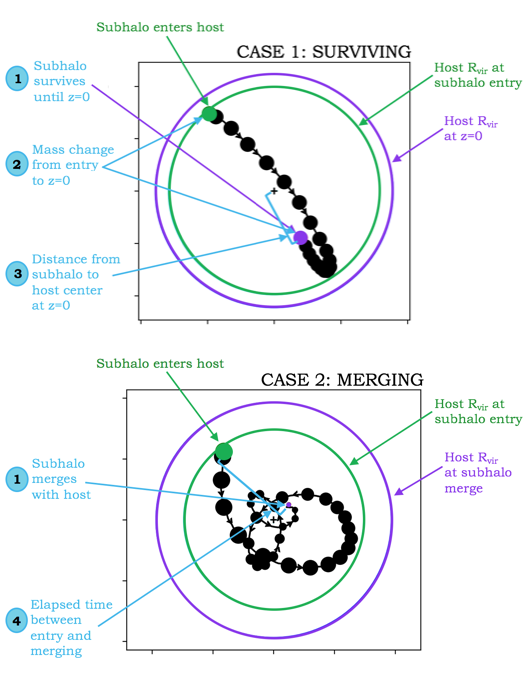
\includegraphics[width=\columnwidth]{Figures/explanatory_figures}
    \caption{An example of a surviving (top) and merging (bottom) interaction between a subhalo and host halo. The orbit of these two subhalos are shown within the virial radius of their respective host halos. Size of points along the orbit correspond to the mass of the subhalo. In order to see the orbits and the size of the points more clearly, we have plotted only every eighth timestep of the subhalo's orbit. Quantities that we try to predict in this work are labeled and numbered in the order they will be presented throughout the paper.}
    \label{fig:explanatory_figures}
\end{figure}

	Our analysis makes use of VISHNU, a cosmological N-body simulation with 1000 snapshots. VISHNU contains 1680\textsuperscript{3} particles in a volume of 130h\textsuperscript{-1} cMpc and uses WMAP-1 cosmology (\citet{Spergel2013}; $\Omega$\textsubscript{m} = 0.25, $\Omega$\textsubscript{$\Lambda$} = 0.75, $\Omega$\textsubscript{b} = 0.04, $\sigma$\textsubscript{8} = 0.8, \textit{n\textsubscript{s}} = 1.0, \textit{h} = 0.7). Each dark matter particle has mass \textit{m\textsubscript{p}} = 3.215 $\times$ 10\textsuperscript{7}h\textsuperscript{-1} M\textsubscript{\(\odot\)}, and subhalos can contain as few as 2 particles. The ROCKSTAR halo finder was used to identify halos and subhalos, and merger trees were constructed with Consistent-Trees (\citet{Behroozi2013b}).
\par
    From the merger trees, we select subhalos of the most massive progenitors of host halos at \textit{z}=0. These subhalos are allowed to have further substructure inside of them but cannot, at any point during their infall, become sub-substructure themselves. To help mitigate resolution uncertainties, we select only subhalos which consist of 1000 particles (total mass 3.215 $\times$ 10\textsuperscript{10}h\textsuperscript{-1} M\textsubscript{\(\odot\)}) or more at their time of accretion. We define the accretion point of a subhalo as the last timestep before a subhalo enters its host. As such, at the initial time of accretion, the will-be subhalos are still host halos themselves. Once the subhalo has entered its host, however, it cannot leave again (so, a flyby interaction would not be considered on its first pass but will be considered on a later pass if it falls back into and remains inside the host). Once it has been accreted, the subhalo must have one of two fates: merge with the host, or remain a bound, identified subhalo within that host until today. Following uncertainties in subhalo mass loss shown by \citet{VDB2018}, once a subhalo has lost more than 90\% of its mass, it is considered to be merged.
\par
    In addition to making cuts for resolution, some merging interactions were removed due to their unphysical behavior, likely as a result of errors in the merger trees. \textbf{INSERT NUMBER} Subhalos were removed that gained more than 10 times their mass (\textit{or some threshold.. I don't know yet what's best yet}) during infall. These subhalos likely had their identifications changed as they moved close to the center of the host. \textbf{INSERT NUMBER} subhalos were removed because their initial mass was larger than that of its supposed host. \textbf{INSERT NUMBER} subhalos were removed because their positions were outside of their host's virial radius after periodic boundary conditions were corrected for. \textbf{INSERT NUMBER} subhalos were removed because their time of merging was earlier than their time of entry?? \textit{Show a few cases of these strange orbits/mass loss histories??}
\par
	Although we have attempted to correct for these errors, there remains the possibility that erroneous cases still exist within our sample. We have made a hard cut to remove halos that gain mass, but there may be still be cases where an identification of a halo was changed within our sample. Possible other cases we found: Weird looking orbits that weren't in initial filtering. Some discussion of the cases that could possibly still exist in the data due to difficulty in being able to filter them out/ find a general way to search for them? \textit{Something that gives some estimation of how many cases might be like this? To ensure that it's not some large part of the sample and the reason we can't predict things. Mention that we removed about 2\% of the total number so even if you assume the same portion is wrong it shouldn't be the source of the stochasticity?}
\par
    Our resulting sample includes a total of \textbf{INSERT NUMBER} subhalo-halo interactions. Distributions of this sample with respect to host masses, mass ratios, and the scale factor of the time of entry are shown in Fig.~\ref{fig:combined_distributions_logBin}. The most common interactions in our sample are mergers of lower mass ratio that occurred more recently. However, our sample also spans the space of more equal mass and higher redshift mergers, with hundreds of interactions shown in many of the bins in Fig.~\ref{fig:combined_distributions_logBin}. \textit{Some reference to how many of these are expected? Indication that this is a representative sample of what we expect to see slash agreement with other simulations?}
\par
    For both the host halo and subhalo at the timestep of infall, and at either the timestep right before merging or at z=0, we take several physically-motivated parameters to describe the interaction between the halos. Table 1 lists these parameters and includes a brief description of each. \textit{Include ALL parameters that we took and then somehow mark the ones that we kept or only mention the ones that we kept. I don't want a table of a billion things but also don't want any question that we didn't cover everything}. From the parameters taken from the merger trees, we calculated some additional parameters. These include the eccentricity, mass ratio (M\textsubscript{ratio}=M\textsubscript{sub}/M\textsubscript{host}), relative distances and relative velocities? \textit{How much to go over these, or do we even need to mention calculating stuff like relative distance because it's so obvious.} Initial parameters, which were used as input parameters to the machine learning models to make predictions, include:
    
    \begin{itemize}
        \item \textbf{a}: the scale factor of the universe at the time of the subhalo's entry.
        \item \textbf{M\textsubscript{sub,i}}: the virial mass of the subhalo at the time of its entry.
        \item \textbf{M\textsubscript{host,i}}: the virial mass of the host halo at the time of the subhalo's entry.
        \item \textbf{M\textsubscript{sub,i}/M\textsubscript{host,i}}: the ratio of subhalo to host halo masses at the time of the subhalo's entry.
        \item \textbf{R\textsubscript{vir,sub,i}}: the virial radius of the subhalo
        \item \textbf{R\textsubscript{vir,host,i}}: the virial radius of the host halo
        \item \textbf{c\textsubscript{sub}}: the concentration of the subhalo
        \item \textbf{c\textsubscript{host}}: the concentration of the host halo
        \item \textbf{\textlambda\textsubscript{sub}}: Bullock spin parameter of the subhalo
        \item \textbf{\textlambda\textsubscript{host}}: Bullock spin parameter of the host halo
        \item \textbf{v\textsubscript{rel}}: relative total velocity between subhalo and host halo, calculated in the reference frame of the sub.
        \item \textbf{d\textsubscript{rel,i}}: relative absolute total distance between subhalo and host halo centers
        \item \textbf{\textepsilon}: eccentricity of subhalos initial orbit
        \item \textbf{max(M\textsubscript{subs,sub})}: the virial mass of the most massive sub-subhalo within the subhalo at the time of the subhalo's entry. 0 if subhalo has no sub-substrucutre.
        \item \textbf{max(M\textsubscript{subs,host})}: the virial mass of the most massive subhalo already within the host halo at the time of the selected subhalo's entry. Does not include the selected subhalo.
        \item \textbf{N\textsubscript{subs,sub}}: the total number of sub-subhalos within the subhalo at the time of entry.
        \item \textbf{N\textsubscript{subs,host}}:  the total number of subhalos within the host halo at the time of entry. Does not include the selected subhalo.
        \item \textbf{T\textsubscript{sub}}: the triaxiality parameter of the subhalo at the time of entry.
        \item \textbf{T\textsubscript{host}}:  the triaxiality parameter of the host halo at the time of entry.
    \end{itemize}
    
    Parameters that are taken at the end of the interaction, either at the time of merging or at z=0, are used to define the quantities that the machine learning models will predict. These parameters include:
    
\renewcommand{\theenumi}{\arabic{enumi}}
    \begin{enumerate}
        \item \textbf{survival}: a 0 or 1, depending on if the subhalo exists above the required mass threshold at z=0 (survives, 1) or if the subhalo has merged with its host at some time before (merges, 0)
        \item \textbf{M\textsubscript{sub,f}}: the virial mass of the subhalo at the end of the interaction.
        \item \textbf{d\textsubscript{rel,f}}: relative absolute total distance between subhalo and host halo centers at the end of the interaction, normalized by the virial radius of the host halo.
        \item \textbf{t\textsubscript{merge}}: the elapsed time between entry of a subhalo into the host virial radius and the time of merging with the host.
    \end{enumerate}
\par
    As preparation for using machine learning, we split the data into train and test sets, with 80\% of the data to be used for training and 20\% to be used for testing. These subsamples are selected randomly from the total sample. \textit{Counts and some simple statistics of these sets are shown in Table 2. Averages and standard deviations of these samples are similar, showing that the test set is representative of the training set.} The data was also scaled and normalized to have a mean of zero and unit variance. For training the machine learning models, the training set was further divided into training and validation sets, also using an 80/20 split. From the original dataset, this means the data was split as 64\% training, 16\% validation, and 20\% testing.

\begin{figure*}[h]
	% To include a figure from a file named example.*
	% Allowable file formats are eps or ps if compiling using latex
	% or pdf, png, jpg if compiling using pdflatex
	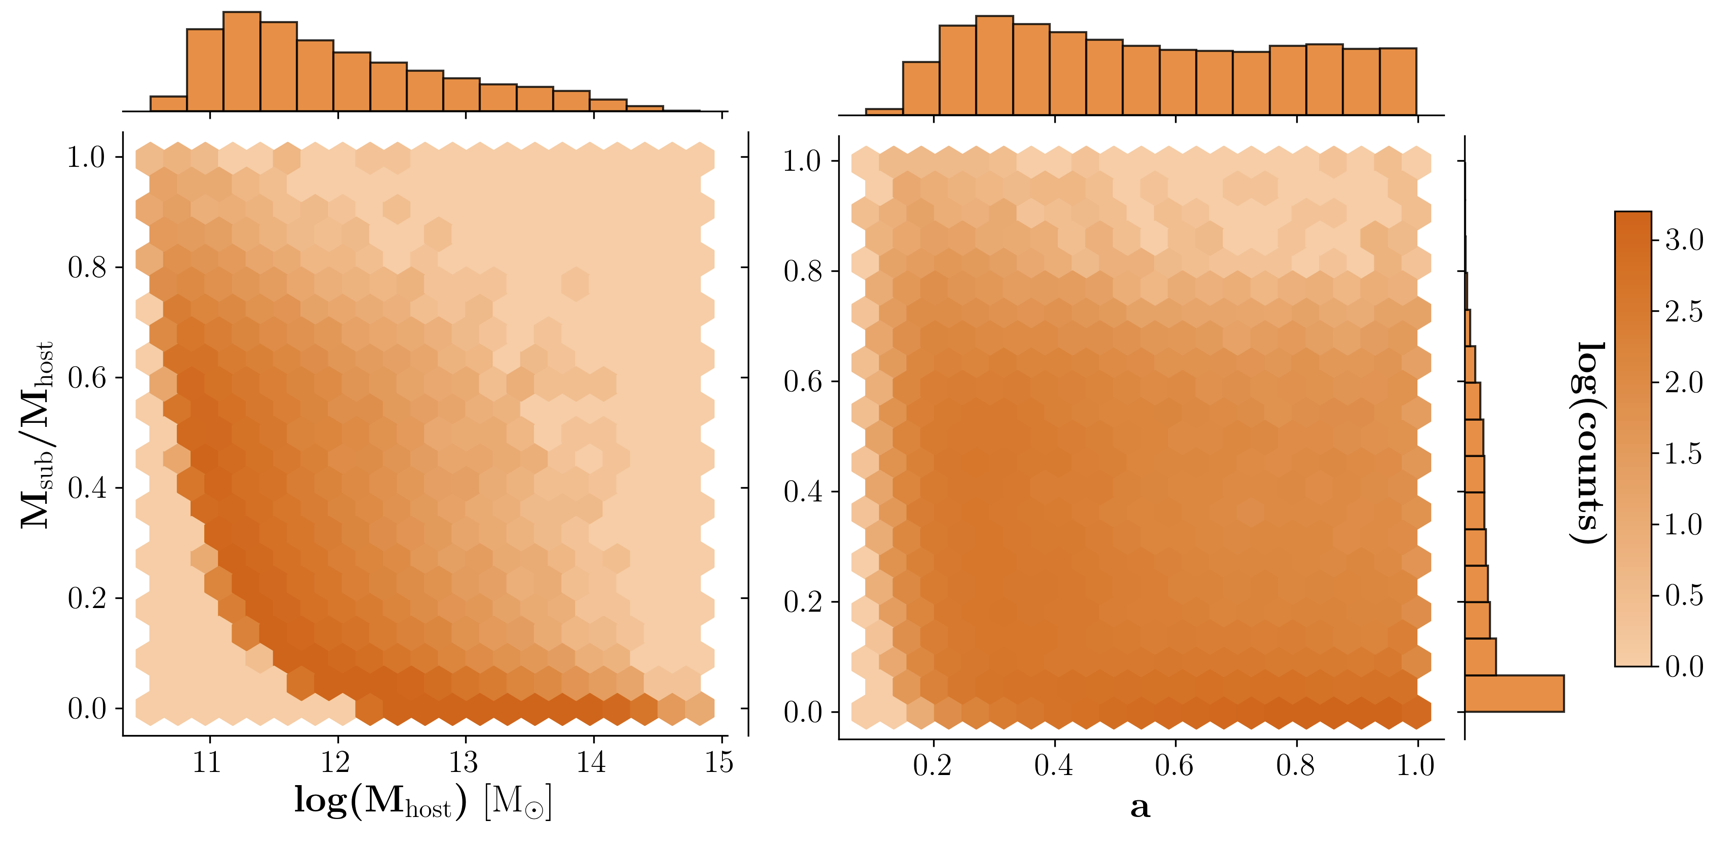
\includegraphics[width=\textwidth]{Figures/combined_distributions_logbin}
    \caption{Distributions of the merging interactions within our sample, in two different two-dimensional spaces. The left panel shows the distribution of mergers in the space of the host mass (x-axis) and the mass ratio (y-axis) of the interaction. The right panel shows the distribution of mergers in the space of the scale of initial entry of the subhalo (x-axis) and again, the mass ratio of the interaction on the y-axis. Within each hexagonal bin, the counts of interactions are shown, on a logarithm scale, by the colorbar. Histograms show the one-dimensional distribution of host masses (above the left panel), scale of entry (above the right panel) and mass ratios to the right of the right panel). Most interactions occur at lower mass ratios and for smaller host halos, but the spaces are still well-spanned over a range of interactions in both panels. }
    \label{fig:combined_distributions_logBin}
\end{figure*}



\section{Machine Learning Methods}
\label{sec:ML Methods}
The machine learning algorithms used in this work come from the \texttt{scikit-learn} package for python. For the classification problem of subhalo survivial, we use the random forest algorithm. For the regression problems of predicting mass loss, final position, and merging time, we use the gradient boosting regressor algorithm. Although the reader is referred to the \texttt{scikit-learn} documentation for a full description of these algorithms, a brief description of these methods is included in this section.

\subsection{Random Forests}
\label{sec:rf} % used for referring to this section from elsewhere
\textit{Basic description of the algorithm and how it works. What parameters are there to play with and what that changes about the way that the model does its thing.} Random forest classifiers use a compilation of decision trees to reach consensus on a prediction. Individual decision trees are trained on random subsets of the dataset, and the majority vote of all decision trees gives the classification. The scikit-learn algorithm uses by default the Gini impurity to measure the goodness of a decision split within each decision tree. There are several hyperparameters of the algorithm that we tune in order to get the best-fitting model. The number of estimators hyperparamter sets the number of decision trees that will be separately trained and used in the final consensus. The depth hyperparameter sets how many decisions can be made going down each tree before reaching a classification decision. The maximum number of nodes hyperparameter sets the maximum number of new nodes an existing node can split into at the next depth level. We keep other parameters of the algorithm set to their default values.

\textit{Advantages and disadvantages.} The advantage of using a random forest over a single decision tree is the reduction of overfitting. Because each decision tree is given some subset of the dataset, and decision splits are made on random subsets of the parameters, individual decision are less overfit and the consensus of the all decision trees is more robust to unseen data. This is important especially in cases like our own where we have a relatively large number of training examples and small number of needed parameters. Unfortunately, the results of a random forest can also be more difficult to interpret than those of more simple classifiers. Because each decision tree only sees some portion of the information, some decision trees may be very poor predictors. The \texttt{scikit-learn} random forest classifier provides a function that ranks the importance of training features given their frequency of selection and proximity to the top of the decision trees. However, strong correlations between features can make this ranking difficult to straightforwardly interpret as well, because features that are important but also strongly correlated with other features may be selected less frequently in lieu of their strongly correlated counterpart.

\textit{Applications to this specific problem.} The subhalo survival classification problem is a binary classification problem, which assigns a subhalo a value of 0 for merging before z=0, and a value of 1 for surviving until z=0. We train the model using all initial features described in \ref{sec:simulation}. Given the strong correlations amongst several of our parameters, we do not use the order of feature importance given by the \texttt{scikit-learn} algorithm to decide which of our features are most prominent, and instead choose our own order, outlined in \ref{sec:feature selection} below. We use this order to train models, using the same hyperparameters, on smaller subsets of the features to confirm the number of features needed to make predictions.

\subsection{Gradient Boosting Regressors}
\label{sec:gbr} % used for referring to this section from elsewhere
\texit{Basic description of the algorithm and how it works.} Gradient boosting regressors use a number of weak learners, like decision trees, along with some measure of how well each tree does to train additional trees. Like random forests, the consensus of many decision trees is the prediction. However, unlike random forests, the results of the trees are additive, rather than majority vote. Thus, gradient descent is performed with the addition of each tree and the loss is minimized. We use a huber loss function as it is shown to be robust.... As with the random forest classifier, several hyperparameters can be tuned to create the best model. The learning rate hyperparameter shrinks the contribution of each additionally added tree to the ensemble, decreasing the contribution of each tree but allowing more improvement to the model. As with the random forest classifier algorithm described above, we also tune the number of estimators, depth, and maximum number of nodes hyperparamters for individual trees in the gradient boosting algorithm. Other parameters of the algorithm are kept as their default values.

\textit{Advantages and disadvantages.} The advantage of using a gradient boosting regressor is that... How easy it can be to overfit given the smaller scope of the problem, dangers of underfitting when trying to trim down parameters. As with the random forest classifier, this gradient boosting regressor class in python also contains a function to report relative feature importances. However, interpreting these results again presents difficulties. How different parameters of the model can constrain the model to only use some features. Advantages over simpler models.

\texit{Applications and such to this specific problem.} For each of our regression problems, we use a gradient boosting regressor to predict the final quantity. A different gradient boosting regression model is created and separately tuned for each of our outcomes we predict. Each model is is given all initial features to train on. As with the survival classification problem, due to the difficulty of interpreting the reported feature importances of the algorithm, we use our custom algorithm to determine the order and relative importance of features for predicting each of our desired quanitites.

\subsection{Other Models}
\label{sec:other models} % used for referring to this section from elsewhere
\textit{Not sure if this really needs to be its own subsection at all, or if casually mentioning this type of stuff in the previous sections is sufficient. I don't have too much to say in this section as of now but I guess it can just be a small section?}
Although we have chosen to use a random forest classifier and gradient boosting regression for our analysis, several other popular machine learning models could be chosen. In particular, neural networks have become increasingly popular for a wide variety of applications, to both classification and regression problems due to their ability to fit to data incredibly well. Several other, arguably more intuitive machine learning algorithms could also be used. The K-nearest-neighbors algorithm, for example, assigns predictions based on the properties of objects that are similar to the object trying to be predicted. To ensure that our model was as well fit and possible without being too overfit, we tried several of such machine learning algorithms before settling on our choices.

In particular, neural networks, random forests, and gradient boosting regressors seem to perform quite similarly. \textit{How much it improved/didn't improve? Specific cases? How much to say here? Reason we went with GBR's for all regressors and an RF for the survival problem?}


\section{Feature Selection}
\label{sec:feature selection} % used for referring to this section from elsewhere
\textit{Description of how we reduced/ordered the features. The variation tree procedure for selecting the features and ordering the first few most important ones. How we decided that of all of the parameters we did and could take, no need for more than a few to make good predictions.}

\textit{How we reduced from like 50 parameters to 20? Or should I not go into detail about that.} Initially, our sample contained \textbf{INSERT NUMBER} parameters (or features) to describe each interaction. These parameters are selected to encompass information about the orbit, environment, and individual properties of both the host and subhalo. Although we begin with a large set of parameters for thoroughness, we expect that not all parameters will be important for predicting our desired quantities. In order to determine which parameters most strongly affect the predicted quantities, we use a feature selection method on all of the parameters that selects four parameters for each predicted quantity that are responsible for the most variation in that quantity. Because our set of parameters has strong correlations between several values, we also aim to use a feature selection method that will minimize correlations in the selected subset of features.

\textit{Description of the variation tree method of selecting the most important parameters.}
To select the subset of features, we begin by binning a predicted quantity by each of the feature parameters. Then, the most important feature parameter is the one with the most variation in average value of the predicted quantity within those bins. The next important parameter is selected by again binning within each parameter, within the existing bins of the firstly selected parameter. We repeat this process until four feature parameters have been selected, at which point bins become to small and noisy to continue binning the data any further. The order of feature importance is the order in which the parameters were selected using this method.
 
 {How it fits with doing machine learning methods that rely on decision trees because the underlying assumptions are similar? Problems with getting too much noise when trying to order beyond 4 parameters. What the metric for amount of variation means and what it tells us.}

The results of the four most important features for each of the predicted quantities are shown in Table \ref{tab:FS_table}. The number next to each parameter represents the strength of variance due to that feature. This number is \textbf{IS...} the normalized maximum variance within bins of that parameter. Some parameters, such as the initial scale factor of entry and the eccentricity of the subhalos orbit, appear as important for all of the predicted quantities. In particular, the initial scale is either the first or second most important parameter for all quantities. \texit{Some discussion of whether or not you can tell at this point that some thing being predicted might need an additional parameter (a fifth) or might do well with only 3 (still high variation compared to noise in the last parameter or last chosen parameter close to noise)?}.

\texit{According to selected features, what do the best 2D spaces look like for the things we want to predict?} Using this ranking of most important features, we look at the values of our predicted quantities within the two-dimensional space of the two parameters most responsible for variations in the outcome. This is shown in Figure \ref{fig:bestSpaces}. From this figure, we can see how strongly the predicted quantities rely on their chosen features. For survival, the two-dimensional space is clearly divided, suggesting that the survival of a subhalo is already well-determined by only two parameters. For the other quantities, this gradient is less defined, suggesting more parameters are needed to make good predictions. In particular, merge time seems to not have much variation, even amongst the two parameters that cause the most variation in its outcome. \texit{Something about how that means we can already tell it might be harder to predict?}

% Feature Selection Table
\begin{table}
	\centering
	\caption{The ranking order of most important features for predicting each of the desired quantities. Values next to the chosen feature represent the normalized maximum variation from binning within that parameter, where higher values indicate the parameter is more strongly responsible for changes in the prediction outcome.}
	\label{tab:FS_table}
	\begin{tabular}{c|cccc} % four columns, alignment for each
		\hline
		rank & Survival & Mass Loss & Final Position & Merge Time\\
		\hline
		1 & a () & R\textsubscript{vir,sub} () & R\textsubscript{vir,host} () & a ()\\
		2 & M\textsubscript{sub}/M\textsubscript{host} () & a () & a () & \textepsilon ()\\
		3 & \textepsilon () & \textepsilon () & M\textsubscript{sub}/M\textsubscript{host} () & M\textsubscript{sub}/M\textsubscript{host} ()\\
		4 & v\textsubscript{rel} () & d\textsubscript{rel} & \textepsilon () & c\textsubscript{sub}\\
		\hline
	\end{tabular}
\end{table}

% Best-spaces figure
\begin{figure*}[h]
	% To include a figure from a file named example.*
	% Allowable file formats are eps or ps if compiling using latex
	% or pdf, png, jpg if compiling using pdflatex
	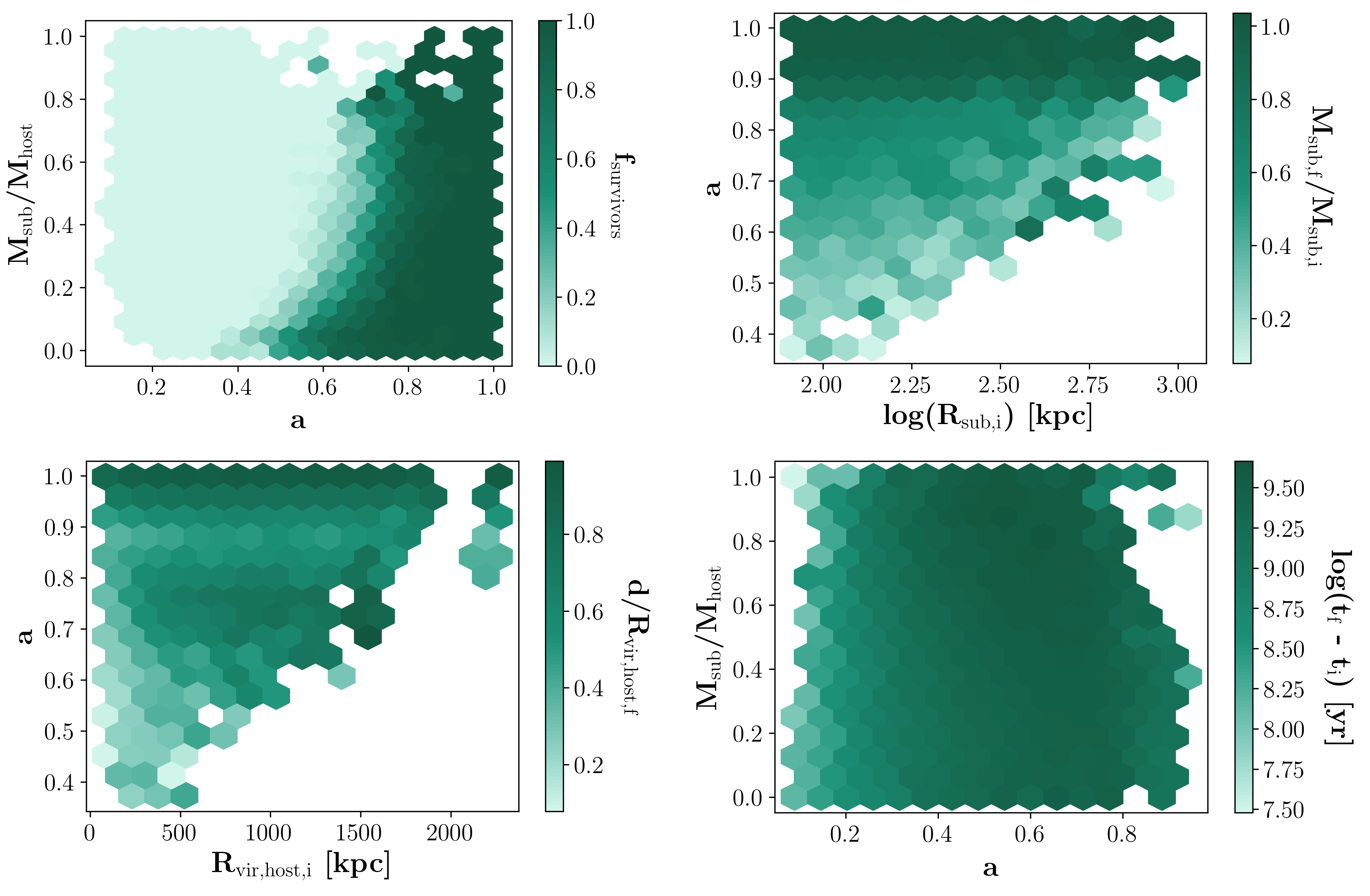
\includegraphics[width=\textwidth]{Figures/bestSpaces}
    \caption{Distributions of the predicted quantity of interest with respect to the two parameters that are most responsible for its variations. In each panel, the parameter that causes the most variation is shown on the x-axis, and the parameter that causes the second most variation is shown on the y-axis. In addition, in each panel the colorbar shows the average values of the quantity of interest within a bin. The top left panel shows the fraction of surviving subhalos. The top right panel shows the fraction of subhalo mass that remains for surviving subhalos. The bottom left panel shows the fractional distance of surviving subhalos from their host's center. The bottom right panel shows the elapsed time for a subhalo to merge. In each instance, some pattern of color striation can be seen to represent the importance of the two parameters shown. However, it is clear that the survival of a subhalo is by far the most drastically divided and well-defined by this two-dimensional space. }
    \label{fig:bestSpaces}
\end{figure*}



\section{Results}
\label{sec:Results}
For each of the final quantities, we train a machine learning algorithm, using all available parameters, to predict the outcome value. For each of quantity, we select hyperparameters of the model by repeatedly training iterations of the model using the training set, and checking its accuracy on the testing set, until the best fit with lowest overfitting is achieved. We also train the same model with the same hyperparameters on smaller subsets of the feature parameters, removing less important parameters, until the model is trained with only the most important parameter from our feature selection methods. In this way, we can determine the minimum subset of parameters needed to achieve maximum accuracy. Section~\ref{sec:survival} discusses this process for predicting the survival quantity. Section~\ref{sec:mass loss} discusses this process for predicting the mass loss quantity, Section~\ref{sec:position} for the final position quantity, and Section~\ref{sec:merge time} does so for the merging time quantity.

\subsection{Survival}
\label{sec:survival} % used for referring to this section from elsewhere
For the entire sample of subhaloes, we first try to predict whether or not a halo will survive until z=0 (1) or merge with the host (0) sometime before z=0 using a random forest classifier. The accuracy metric we use is a straightforward categorical accuracy, which is given as the percentage of halos correctly classified as either 0 or 1.

Figure \ref{fig:survival_predictions} shows the accuracy of best-fit model, when trained using all and increasingly small subsets of the feature parameters. The maximum accuracy reached by this model is 96.5\percent for both the training and testing sets. Although the training set generally does better than the test set, the accuracy difference is small and likely caused by a natural amount of overfitting. This maximum accuracy is achieved using only the three top-ranking parameters, after which the addition of more parameters causes increases or decreases in the accuracy that are within noise. Because the model is free at any iteration to use as many of the provided parameters as needed, this suggests that only these three parameters are necessary to predict the survival of a subhalo.

The three parameters that are needed to achieve this maximum accuracy are: the initial scale of subhalo entry, the mass ratio of subhalo to host halo virial mass, and the eccentricity of the subhalo orbit. With the addition of each of these parameters, a \textbf{INSERT NUMBER}, \textbf{INSERT NUMBER}, and  \textbf{INSERT NUMBER} accuracy percentage is gained for each parameter added, respectively. Within the parameter spaces of the four top parameters, we show in Figure \ref{fig:survival_contours} where the accurately and inaccurately predicted subhalos lie. There is a clear tendency for subhalos with a\textsubscript{i} =  .6 - .7 to be the most difficult to predict. This agrees with the upper left plot of Figure \ref{fig:bestSpaces}, where a clear division between always surviving and always merging occurs at this value. We note that, although most of the poorly predicted halos exist in this small section of parameter space, \textbf{INSERT NUMBER} percent of halos with a\textsubscript{i} =  .6 - .7 are still accurately predicted.

\begin{figure}
	% To include a figure from a file named example.*
	% Allowable file formats are eps or ps if compiling using latex
	% or pdf, png, jpg if compiling using pdflatex
	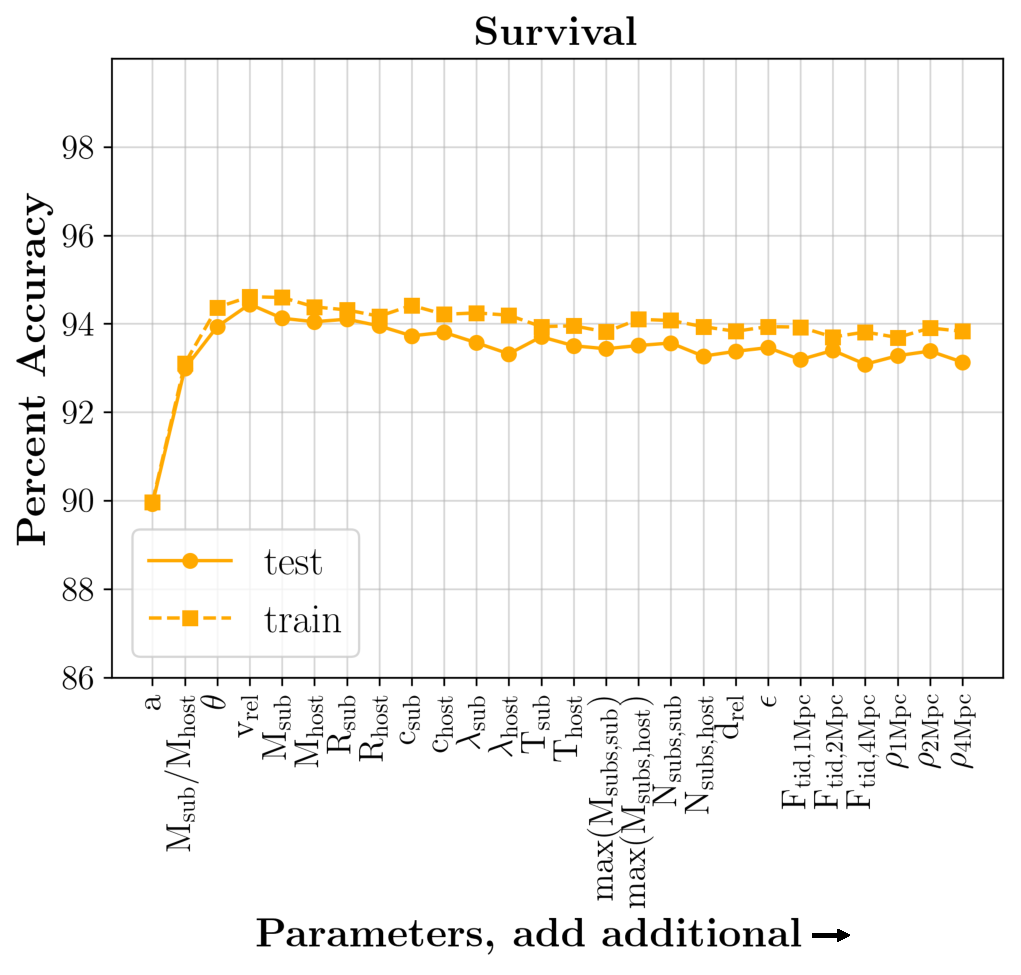
\includegraphics[width=\columnwidth]{Figures/survival_predictions}
    \caption{Accuracy of model's predictions, for both the training and testing sets, when predicting survival. Percentage of the subhalo sample that is predicted accurately is shown on the y-axis. On the x-axis, the parameters used to train the model are shown. For each point, the model was trained using all parameters to the left of that point on the y-axis. The solid line shows the accuracy on the test set, while the dashed line shows the accuracy on the set the model was trained on.}
    \label{fig:survival_predictions}
\end{figure}

\begin{figure*}
	% To include a figure from a file named example.*
	% Allowable file formats are eps or ps if compiling using latex
	% or pdf, png, jpg if compiling using pdflatex
	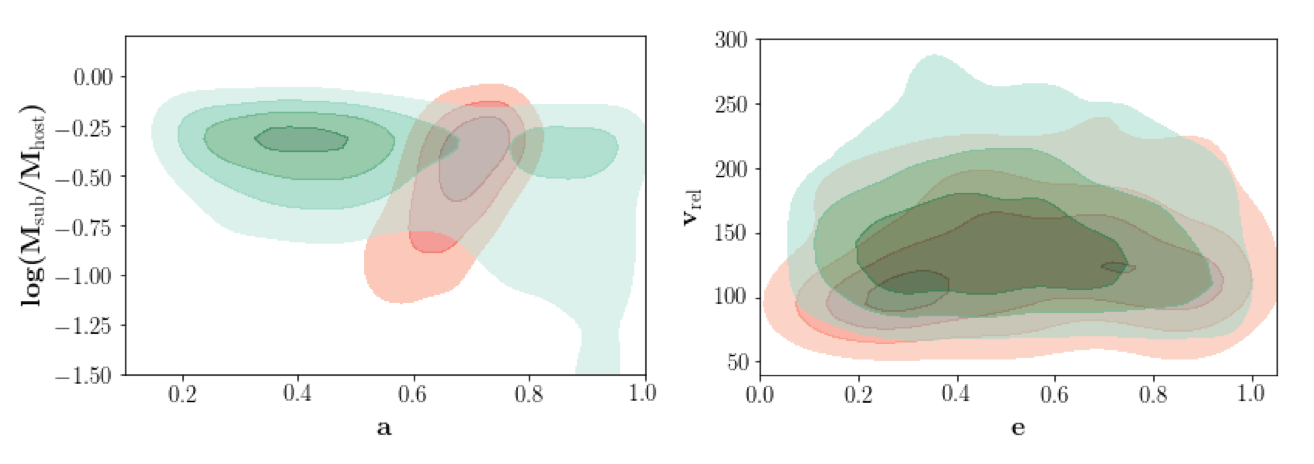
\includegraphics[width=\textwidth]{Figures/survival_contours}
    \caption{Contours of the accurately and inaccurately predicted subhalos, in the two-dimensional spaces of the four most important features. Blue contours show the correctly predicted subhalos, and red contours show the incorrectly predicted subhalos. Contours are divided into 5 sections, with 20\% of subhalos lying within the inner most contour, 40\% lying within the second innermost contour, and so on. The outermost contour is not shaded as to more clearly show the contour regions.}
    \label{fig:survival_contours}
\end{figure*}

\subsection{Mass Loss}
\label{sec:mass loss}
For only subhalos that survive until z=0 without being disrupted, we then predict the mass of the subhalo at z=0 using a gradient boosting regressor. To determine the accuracy of the model, we define an accuracy metric, using the the difference between true and predicted mass fraction. A subhalo is considered to be accurately predicted given:
\begin{equation}
    \label{eq:mass loss}
    \frac{|M_\textsubscript{pred,f} - M_\textsubscript{true,f}|}{M_\textsubscript{true,i}} - \frac{2m\textsubscript{p}\sqrt{N\textsubscript{p,true,i}}}{M_\textsubscript{true,i}} \leq tol
\end{equation}
Where \texit{tol} is some tolerance value which determines what difference in fractional mass loss is acceptable as accurate. The second term in the equation is an additional tolerance, to account for poisson noise in the number of particles assigned to the subhalo.

Figure \ref{fig:massloss_predictions} shows the accuracy of best-fit model, when trained using all and increasingly small subsets of the feature parameters. Because accuracy of this model depends on the selected tolerance value, we show the accuracy given several different choices of tolerance. Again, the training set generally does better than the test set, for all tolerances, due to slight  overfitting. It can be seen that, again using only the three top-ranking parameters, 60\% of subhalos can be predicted to \textpm 5\% of their true final mass. 90\% of subhalos can be predicted accurately, given their prediction requires accuracy to only \textpm 20\% of their final mass. Almost all subhalos can have their masses predicted to within \textpm 50\% of their final fractional mass, although it's worth noting that this encompasses the full range of losing none to all of the original subhalo mass. 

The three parameters needed before prediction accuracy levels off with the addition of more parameters are: the virial radius of the subhalo, the initial scale factor, and the subhalos orbital eccentricity. Again, given the ordering from the feature selection methods discussed above, these parameters show the quickest gain of information with the quickest leveling off of additional accuracy, even given a model allowed to select any of the full twenty parameter set. Adding these first three parameters results in an increase of \textbf{INSERT NUMBER}, \textbf{INSERT NUMBER}, and  \textbf{INSERT NUMBER} accuracy percentage gain, respectively. Within the parameter spaces of the four top parameters, we show in Figure \ref{fig:massloss_contours} where the best and worst 25\% of predicted subhalos lie. Most of the best-predicted subhalos are those that enter their host closer to z=0, likely because those lose much less mass. Larger subhalos, given by larger virial radii, also appear more difficult to predict than their smaller counterparts.  

\begin{figure}
	% To include a figure from a file named example.*
	% Allowable file formats are eps or ps if compiling using latex
	% or pdf, png, jpg if compiling using pdflatex
	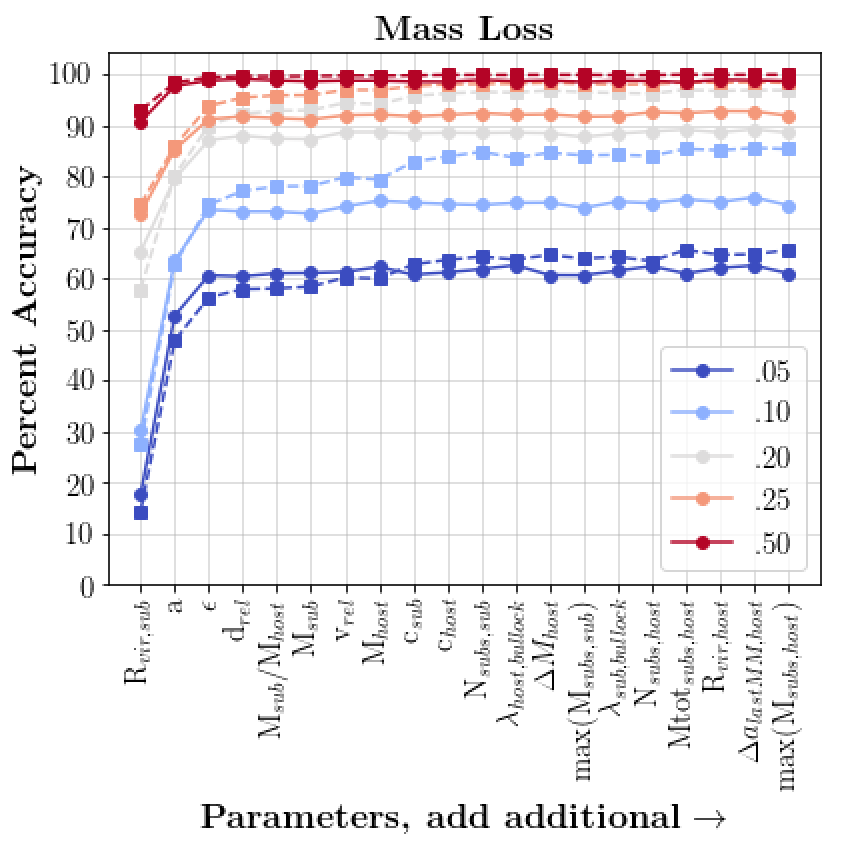
\includegraphics[width=\columnwidth]{Figures/massloss_predictions}
    \caption{Accuracy of model's predictions, for both the training and testing sets, when predicting mass loss. Percentage of accurate predictions is shown on the y-axis. The x-axis shows parameters used to train the model. For each point, the model was trained using all parameters to the left of that point on the y-axis. The solid line shows the accuracy on the test set, while the dashed line shows the accuracy on the set the model was trained on. Different colored lines show the different tolerance values used to define accuracy. For a complete definition of this accuracy metric, see text.}
    \label{fig:massloss_predictions}
\end{figure}

\begin{figure*}
	% To include a figure from a file named example.*
	% Allowable file formats are eps or ps if compiling using latex
	% or pdf, png, jpg if compiling using pdflatex
	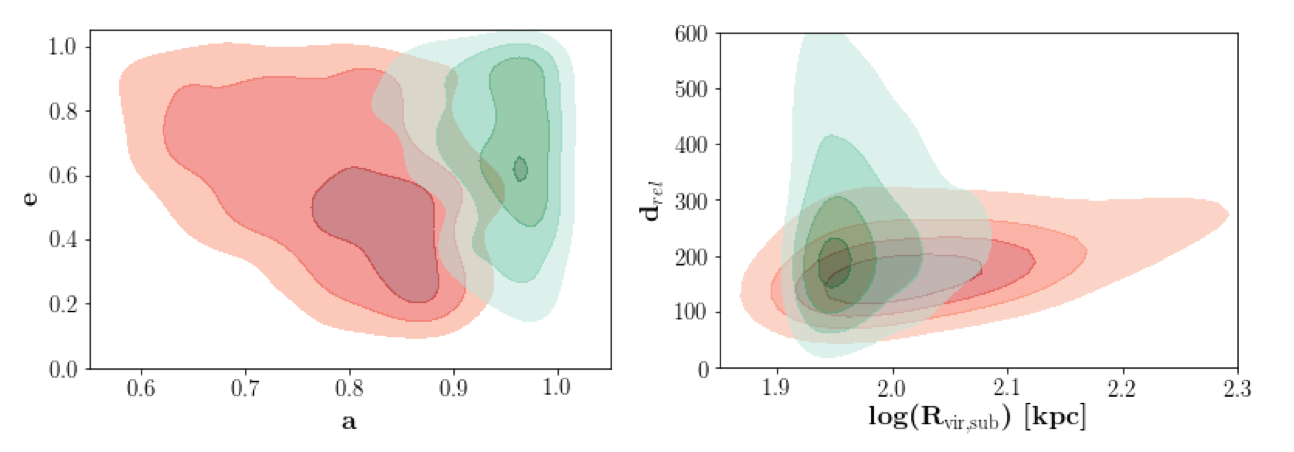
\includegraphics[width=\textwidth]{Figures/massloss_contours}
    \caption{Contours of the top and bottom 25\% accuracies of predicted subhalos, in the two-dimensional spaces of the four most important features. Blue contours show the best predicted subhalos, and red contours show the worst predicted subhalos. Contours are divided into 5 sections, with 20\% of subhalos lying within the inner most contour, 40\% lying within the second innermost contour, and so on. The outermost contour is not shaded as to more clearly show the contour regions.}
    \label{fig:massloss_contours}
\end{figure*}

\subsection{Final Position}
\label{sec:position}
For only subhalos that survive until z=0 without being disrupted, we next predict the final position of the subhalo at z=0, relative to the center of the host halo, using a gradient boosting regressor. To determine the accuracy of the model, we define an accuracy metric, using the the difference between true and predicted fractional distance from host center. A subhalo is considered to be accurately predicted given:
\begin{equation}
    \label{eq:position}
    \frac{|d_\textsubscript{rel,f,true} - d_\textsubscript{rel,f,pred}|}{R_\textsubscript{vir,host,f}} - \frac{2R\textsubscript{soft}}{R_\textsubscript{vir,host,f}} \leq tol
\end{equation}
Where \texit{tol} is some tolerance value which determines what difference in fractional distance from host center is acceptable as accurate. The second term in the equation is an additional tolerance, to account for uncertainty in positions due to the softening length.

Figure \ref{fig:position_predictions} shows the accuracy of best-fit model, when trained using all and increasingly small subsets of the feature parameters. Because accuracy of this model depends on the selected tolerance value, we show the accuracy given several different choices of tolerance. Again, the training set generally does better than the test set, for all tolerances, due to slight  overfitting. For final position, it appears that more parameters are needed to reach maximum accuracy, with the first five given parameters being used for predictions before accuracy levels off. For final position, predictions are slightly worse than for mass loss. 50\% of subhalos can be predicted to \textpm 5\% of their true fractional distance. 90\% of subhalos can be predicted accurately, given their prediction requires accuracy to only \textpm 20\% of their final position. Almost all subhalos can have their final position predicted to within \textpm 50\% of their final fractional mass. Again, we note that this encompasses the full range of the subhalo lying anywhere within the host.

The five parameters needed before prediction accuracy levels off with the addition of more parameters are: the virial radius of the host halo, the initial scale factor, the mass ratio between the sub and host halo, the subhalos orbital eccentricity, and the relative velocity with which the subhalo enters. Given the ordering from the feature selection methods discussed above, it appears that these parameters were chosen to be quite important, although the mass ratio provides less accuracy gain than some of the other, later-chosen parameters. Adding these first five parameters results in an increase of \textbf{INSERT NUMBER}, \textbf{INSERT NUMBER}, \textbf{INSERT NUMBER}, \textbf{INSERT NUMBER}, and  \textbf{INSERT NUMBER} accuracy percentage gain, respectively. Within the parameter spaces of the four top parameters, we show in Figure \ref{fig:position_contours} where the best and worst 25\% of predicted subhalos lie. Most of the best-predicted subhalos are those that enter their host closer to z=0, likely because those have less time to move deep into the host and have their orbits altered as much. 

\begin{figure}
	% To include a figure from a file named example.*
	% Allowable file formats are eps or ps if compiling using latex
	% or pdf, png, jpg if compiling using pdflatex
	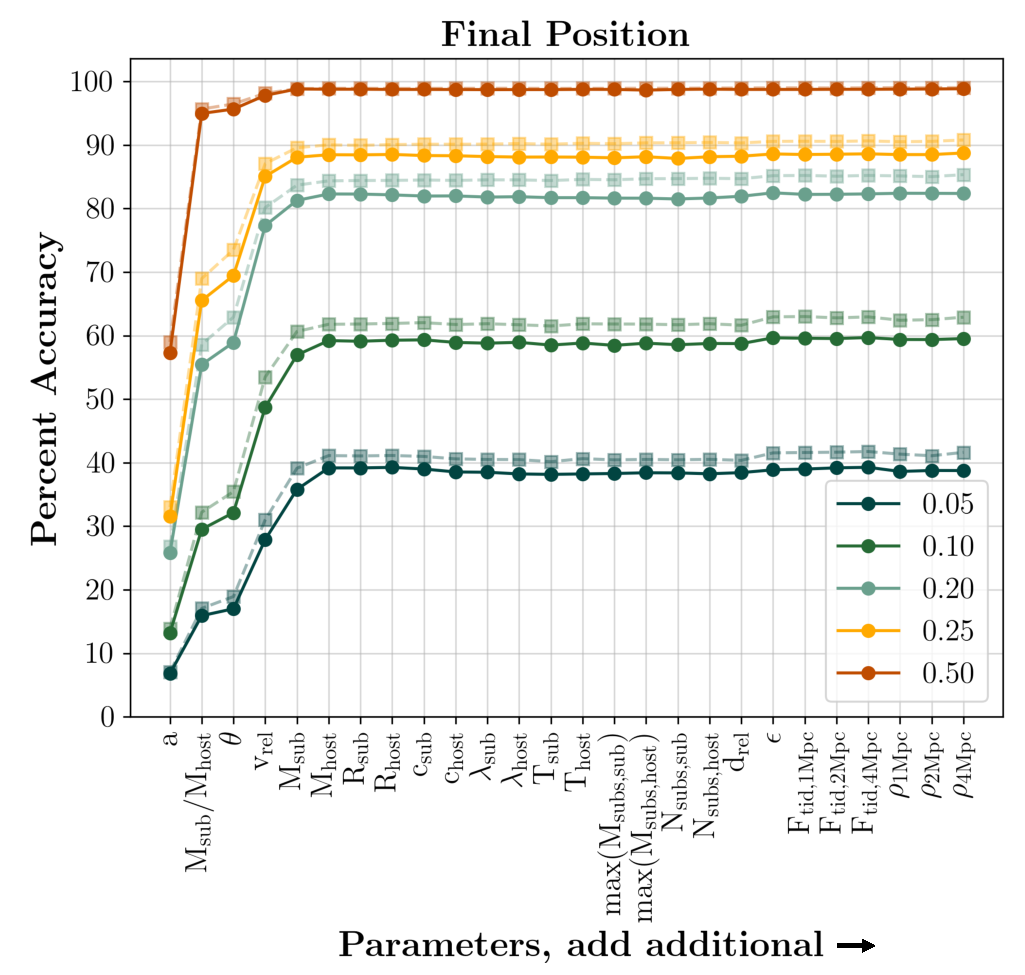
\includegraphics[width=\columnwidth]{Figures/position_predictions}
    \caption{Same as Figure \ref{fig:massloss_predictions}, but for the final position prediction.}
    \label{fig:position_predictions}
\end{figure}

\begin{figure*}
	% To include a figure from a file named example.*
	% Allowable file formats are eps or ps if compiling using latex
	% or pdf, png, jpg if compiling using pdflatex
	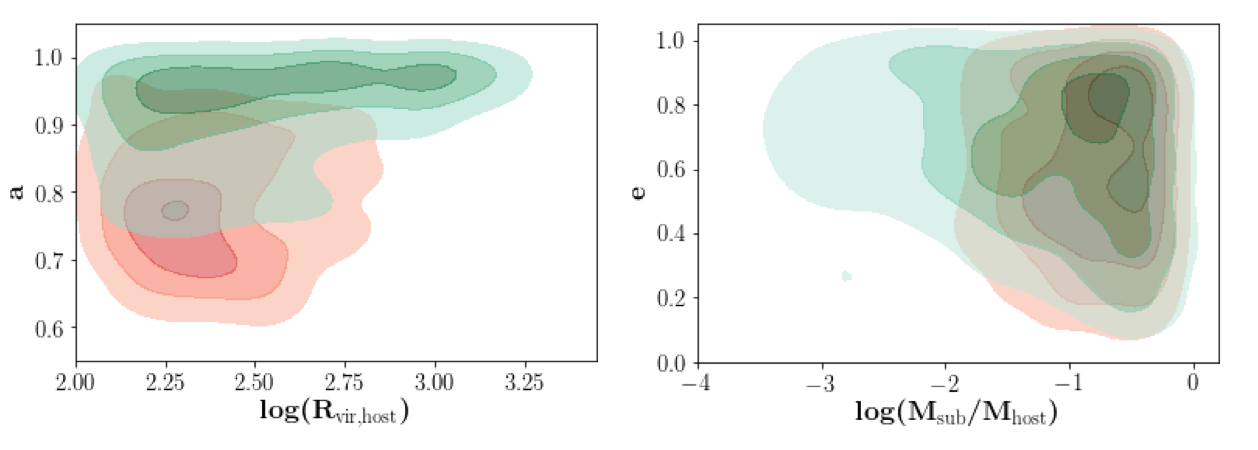
\includegraphics[width=\textwidth]{Figures/position_contours}
    \caption{Same as \ref{fig:massloss_contours}, but for the final position parameters and predictions.}
    \label{fig:position_contours}
\end{figure*}

\subsection{Merge Time}
\label{sec:merge time}
For only subhalos that have merged before z=0, we finally predict the amount of elapsed time between the subhalos entry and subsequent merging, using a gradient boosting regressor. To determine the accuracy of the model, we define an accuracy metric, using the the difference between true and predicted number of crossing times. A subhalo is considered to be accurately predicted given:
\begin{equation}
    \label{eq:position}
    \frac{|t_\textsubscript{f,true} - t_\textsubscript{f,pred}|}{t_\textsubscript{cross,f,true}} \leq tol
\end{equation}
Where \texit{tol} is some tolerance value which determines to witihin how many crossing times a prediction is considered to be accurate.

Figure \ref{fig:time_predictions} shows the accuracy of best-fit model, when trained using all and increasingly small subsets of the feature parameters. Because accuracy of this model depends on the selected tolerance value, we show the accuracy given several different choices of tolerance. Again, the training set generally does better than the test set, for all tolerances, due to slight  overfitting. To predict merging time, again only three parameters appear to be necessary to reach maximum accuracy. 50\% of subhalos can be predicted to within half of a crossing time. 90\% of subhalos can be predicted accurately, given their prediction requires accuracy to only within 1.5 crossing times. All subhalos can have their merging time predicted to within five crossing times. Again, we emphasize that 5 crossing times is typically around 1 billion years.

The three parameters needed before prediction accuracy levels off with the addition of more parameters are: the initial scale factor, the subhalos orbital eccentricity, and the mass ratio between the sub and host halo. Adding these first three parameters results in an increase of \textbf{INSERT NUMBER}, \textbf{INSERT NUMBER}, and  \textbf{INSERT NUMBER} accuracy percentage gain, respectively. Within the parameter spaces of the four top parameters, we show in Figure \ref{fig:position_contours} where the best and worst 25\% of predicted subhalos lie. Most of the best-predicted subhalos have masses more similar to their host halos. The worst-predicted subhalos also appear to have lower concentrations than their better-predicted counterparts. 

\begin{figure}
	% To include a figure from a file named example.*
	% Allowable file formats are eps or ps if compiling using latex
	% or pdf, png, jpg if compiling using pdflatex
	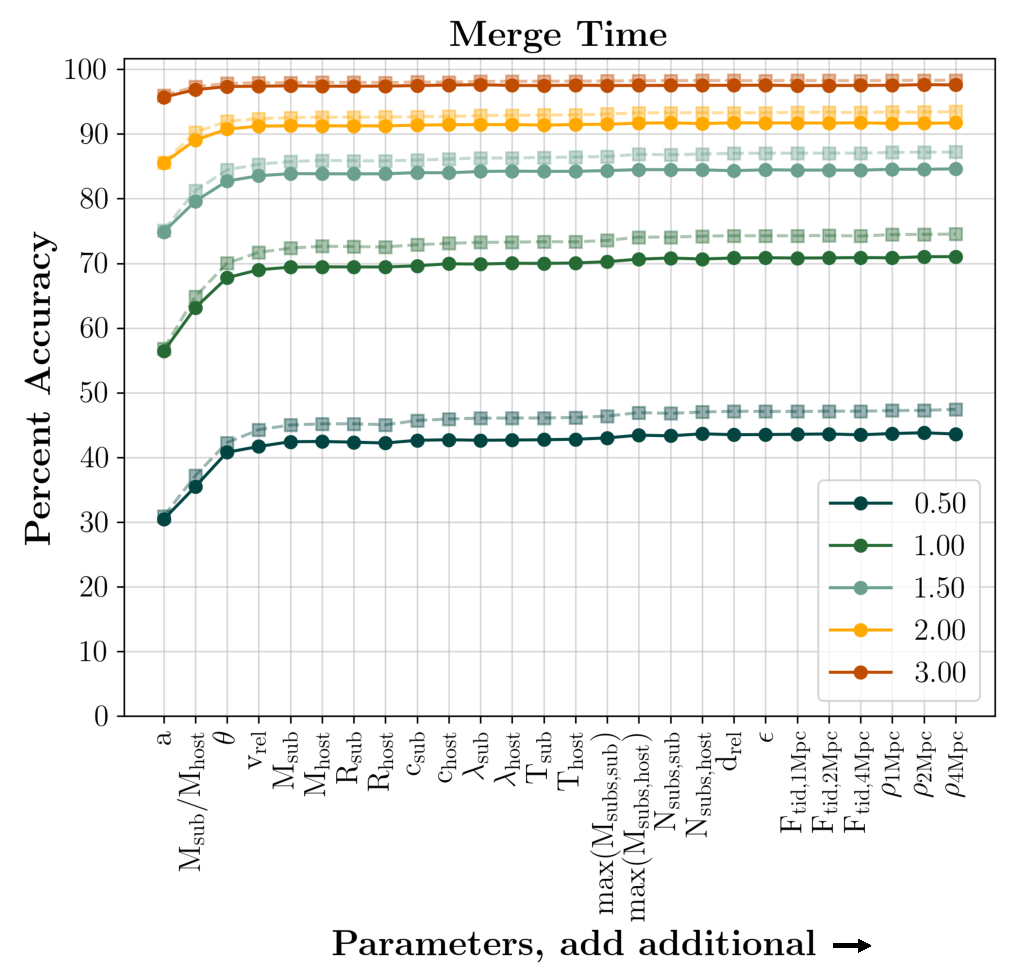
\includegraphics[width=\columnwidth]{Figures/time_predictions}
    \caption{Same as Figure \ref{fig:massloss_predictions}, but for the final position prediction.}
    \label{fig:time_predictions}
\end{figure}

\begin{figure*}
	% To include a figure from a file named example.*
	% Allowable file formats are eps or ps if compiling using latex
	% or pdf, png, jpg if compiling using pdflatex
	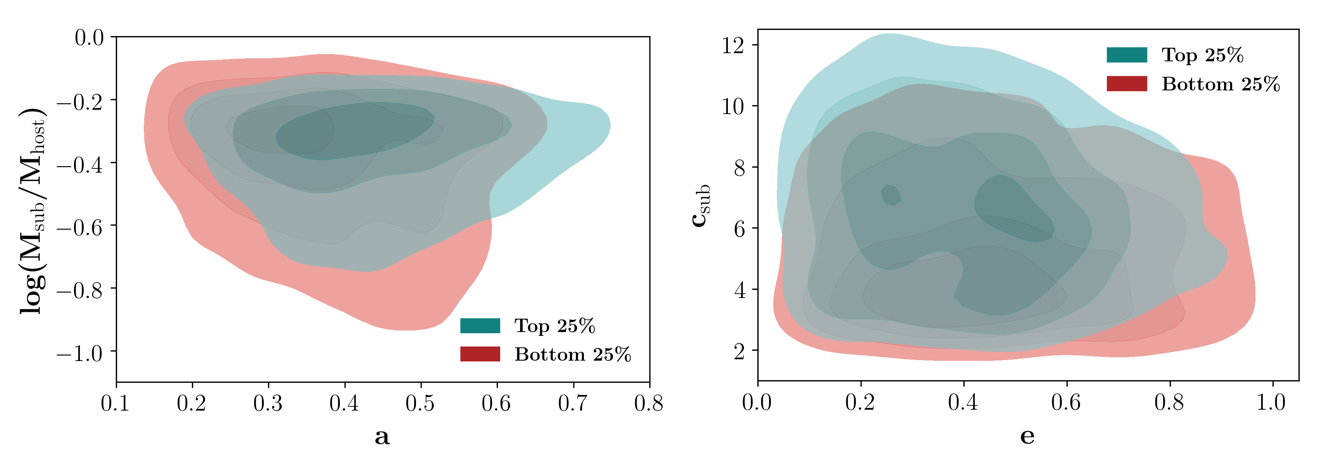
\includegraphics[width=\textwidth]{Figures/time_contours}
    \caption{Same as \ref{fig:massloss_contours}, but for the merge time parameters and predictions.}
    \label{fig:time_contours}
\end{figure*}


\section{Discussion and Summary}
\label{sec:Conclusion}

In this paper, we have used machine learning algorithms to fit a model that predicts the survivial, mass loss, final position, and merge time of a subhalo from parameters taken right at the time of its infall. Our goals were to better understand to what degree these final outcomes are due to stochasticity in subhalo evolution versus real, physically-motivated processes that could be consistently, analytically predicted. From predictions based on these models, we have found:
\begin{itemize}
    \item Subhalo survival can be predicted remarkably well, with 96.5\% of our sample being correctly predicted as surviving or disrupting. These predictions need only three initial parameters: the scale factor at the time of the start of the interaction, the mass ratio between the subhalo and its host, and the orbital eccentricity, but the initial scale factor is by far the most influential of these parameters. Subhalos with both late and early entry times are easiest to predict, while those entering their host halos at a = ~.65 are much more difficult.
    \item Subhalo mass loss is, a generally stochastic process. Although 60\% of our sample can be correctly predicted to within 5\% of their initial masses, an accuracy of 90\% is only achieved given predictions are accurate to within 20\% of their initial mass. These predictions also need only three initial parameters: the virial radius of the subhalo, the scale factor at the time of the start of the interaction, and the orbital eccentricity. Smaller subhalos with late entry times are easier to predict than their larger or earlier counterparts.
    \item Subhalo final locations are also difficult to predict. 50\% of our sample can be correctly predicted to within \textpm 5\% of their the host virial radius, but an accuracy of 90\% is only achieved given predictions are accurate to within 20\% of the host virial radius. These predictions need five initial parameters: the virial radius of the host halo, the scale factor at the time of the start of the interaction, the mass ratio between the sub and host halo, the orbital eccentricity, and the initial relative velocity.
    \item Subhalo merging timescales are also difficult to predict. 50\% of our sample can be correctly predicted to within half of their initial crossing time, but an accuracy of 90\% is only achieved given predictions are accurate to within 1.5 crossing times. These predictions again need only three parameters: the scale factor at the time of the start of the interaction, the orbital eccentricity, and the mass ratio between the sub and host halo. 
\end{itemize}

What went wrong for the outcomes that can't be predicted very well. Show/Discuss specific cases where outcomes are predicted well/not well? Show the contour plots here? Talk about if there are any common spaces within those contours that are consistently not predicted well. Like things in a mid-scale range (.6) being predicted poorly for pretty much anything you want to know. Is there anything common amongst the halos that are predicted poorly for different parameters (are the same haloes or types of halos predicted poorly across multiple outcomes).

\texit{Possible missing parameters.} Anything else that might contribute to the predictions that we haven't included. What do the distributions in parameter space tell us about the ML failing to capture information vs the outcomes having some inherent randomness.

\texit{Robustness of the machine learning results.} Investigation of data size to show that we weren't constrained by amount of data. Cost curves during training? ROC curves? Is it possible the model could have done better given a different tuning/training of the ML algorithms? Discussion of possible underfitting/overfitting of the models. Room for improvement in the ML methodology.

\textit{Possible uses or implications of the models for simulation.} What does this inherent stochasticity seem to point to? What can we say about the results of simulations or how they do their calculations of these types of merging interactions based on the uncertainty in the outcomes of the objects? How much can we expect this type of uncertainty and is it a cause for concern.

\textit{Possible use/implications for observation} Is there anything we can say about distributions that we can expect around the MW or other galaxies. Particularly for survival which we obviously predict much better than the other quantities.

Discussion of future works related to this??


\begin{figure*}
	% To include a figure from a file named example.*
	% Allowable file formats are eps or ps if compiling using latex
	% or pdf, png, jpg if compiling using pdflatex
	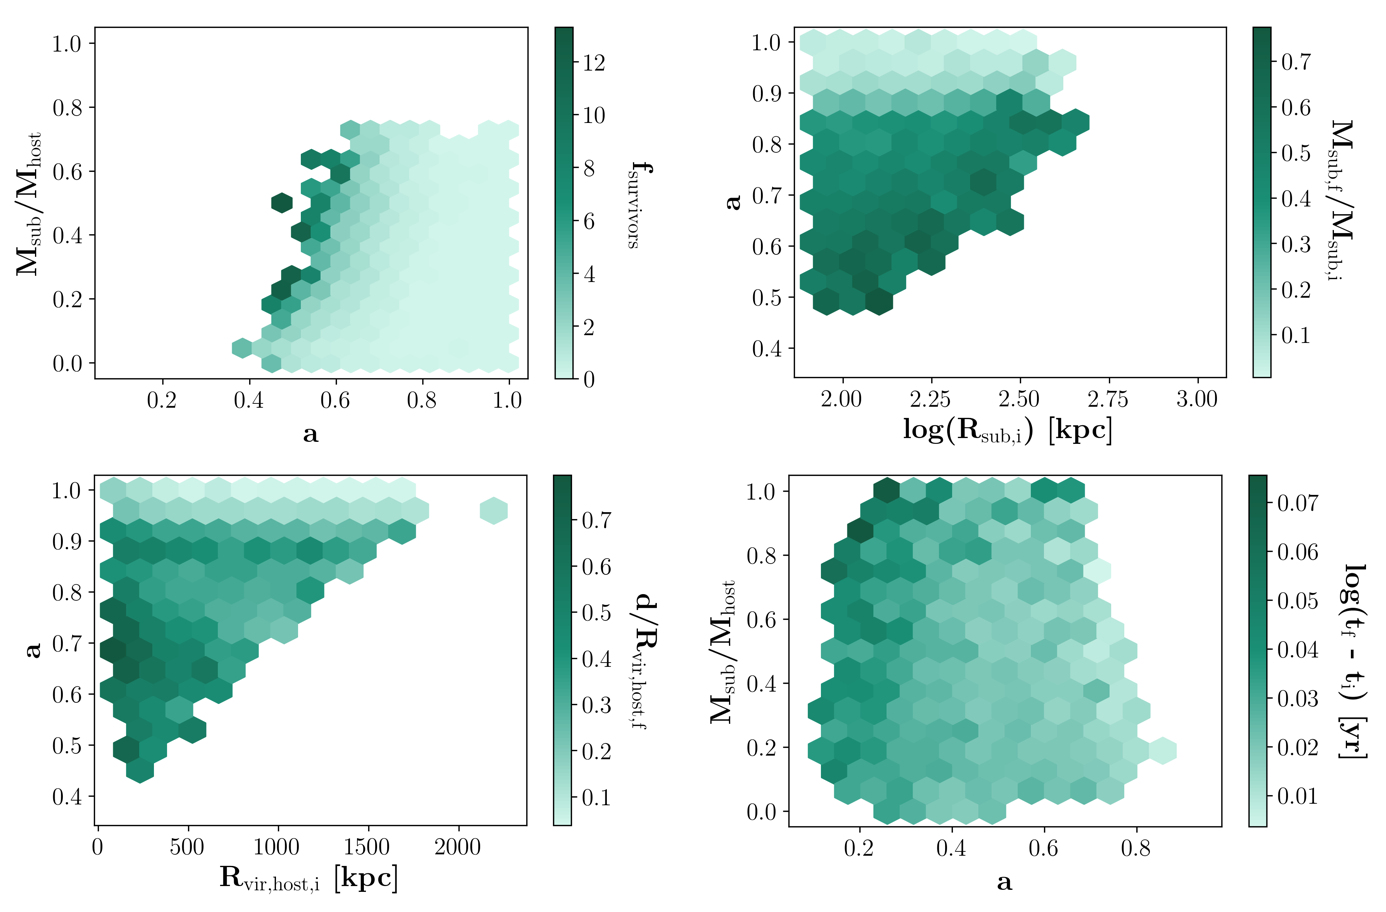
\includegraphics[width=\textwidth]{Figures/stdev_bestSpaces}
    \caption{Same as Figure \ref{fig:bestSpaces}, but each hexagonal bin contains the average standard deviation, normalized by the average value within that bin.}
    \label{fig:stdev_bestSpaces}
\end{figure*}

\section*{Acknowledgements}

I would like to thank the academy, ...

%%%%%%%%%%%%%%%%%%%%%%%%%%%%%%%%%%%%%%%%%%%%%%%%%%

%%%%%%%%%%%%%%%%%%%% REFERENCES %%%%%%%%%%%%%%%%%%

% The best way to enter references is to use BibTeX:

%\bibliographystyle{mnras}
%\bibliography{example} % if your bibtex file is called example.bib


% Alternatively you could enter them by hand, like this:
% This method is tedious and prone to error if you have lots of references
\begin{thebibliography}{99}
\bibitem[\protect\citeauthoryear{Spergel}{2013}]{Spergel2003}
Spergel A.~N., OtherStuff NotReal. 2003, Journal of Improbable Astronomy, 1, 1
\bibitem[\protect\citeauthoryear{Behroozi}{2013}]{Behroozi2013b}
Behroozi A.~N., OtherStuff NotReal. 2013, Journal of Improbable Astronomy, 1, 1
\bibitem[\protect\citeauthoryear{van den Bosch et al.}{2018}]{VDB2018}
van den Bosch A.~N., OtherStuff NotReal. 2018, Journal of Improbable Astronomy, 1, 1
\bibitem[\protect\citeauthoryear{van den Bosch}{2017}]{VDB2017}
van den Bosch A.~N., OtherStuff NotReal. 2017, Journal of Improbable Astronomy, 1, 1
\bibitem[\protect\citeauthoryear{van den Bosch et al.}{2016}]{VDB2016}
van den Bosch A.~N., OtherStuff NotReal. 2016, Journal of Improbable Astronomy, 1, 1
\bibitem[\protect\citeauthoryear{Avila et al.}{2013}]{Avila2013}
Avila A.~N., OtherStuff NotReal. 2016, Journal of Improbable Astronomy, 1, 1
\bibitem[\protect\citeauthoryear{Knebe et al.}{2011}]{Knebe2011}
Knebe A.~N., OtherStuff NotReal. 2016, Journal of Improbable Astronomy, 1, 1
\bibitem[\protect\citeauthoryear{Srisawat et
al.}{2013}]{Srisawat2013}
Srisawat A.~N., OtherStuff NotReal. 2016, Journal of Improbable Astronomy, 1, 1
\bibitem[\protect\citeauthoryear{Nadler et al.}{2017}]{Nadler2017}
Nadler A.~N., OtherStuff NotReal. 2016, Journal of Improbable Astronomy, 1, 1
\end{thebibliography}

%%%%%%%%%%%%%%%%%%%%%%%%%%%%%%%%%%%%%%%%%%%%%%%%%%

%%%%%%%%%%%%%%%%% APPENDICES %%%%%%%%%%%%%%%%%%%%%

\appendix

\section{Some extra material}

If I wanted to present additional material which would interrupt the flow of the main paper, that would go here.

%%%%%%%%%%%%%%%%%%%%%%%%%%%%%%%%%%%%%%%%%%%%%%%%%%


% Don't change these lines
\bsp	% typesetting comment
\label{lastpage}
\end{document}

% End of mnras_template.tex